% Adapted by M-L. Messai
\documentclass[25pt, a0paper, portrait, margin=0mm, innermargin=15mm,blockverticalspace=15mm, colspace=15mm, subcolspace=8mm]{tikzposter}

\usepackage{pgfplots}
\usepackage{booktabs}
\usepackage{multirow}
\usepackage{capt-of}

\usepackage[utf8]{inputenc}
\renewcommand{\refname}{Références}
\usepackage{lipsum} 
\usepackage{fancyhdr}
\usepackage[scaled]{helvet}
\renewcommand\familydefault{\sfdefault} 
\usepackage[T1]{fontenc}
\usepackage{transparent} % transparence des images

\usepackage{soulutf8} % surligner du texte
%\sethlcolor{} % couleur du surlignage

\usepackage[backend=biber,
    style=numeric-comp,
    maxcitenames=1,
    maxbibnames=1,
    %backref=true
    ]{biblatex}

\usepackage{colortbl} % colorer ligne d'un tableau
\usepackage{xspace}

\usepackage{tikz}
\usetikzlibrary{arrows,shapes}

\usepackage{enumitem} % changer les points de itemize


\tikzposterlatexaffectionproofoff %enlever phrase en bas à droite
\usetheme{Simple} %différents thèmes tikzposter

% ---- Couleurs
\definecolor{mypink1}{rgb}{0.858, 0.188, 0.478}
\definecolor{titlecolor}{RGB}{74, 114, 159}
\definecolor{titledarkcolor}{RGB}{51,102,153}
\definecolor{LightGrey}{RGB}{232, 232, 232}
\definecolor{Grey}{RGB}{222, 223, 225}
\definecolor{DarkerGrey}{RGB}{215,217,219}
\definecolor{FontColor}{RGB}{131,136,138}
\definecolor{Red}{RGB}{204,0,0}
%\definecolor{L-lig}{RGB}{25,124,192}
%\definecolor{eric-lab}{RGB}{54,104,163}
\definecolor{eric-lab}{RGB}{255,73,1} 
\definecolor{eric}{RGB}{255,255,255}



\definecolor{Orange}{RGB}{240,163,10} %ERIC orange
\definecolor{Gray}{RGB}{186,200,211}
\definecolor{LightRed}{RGB}{214,98,93}
\definecolor{LightBlue}{RGB}{160,200,217}
\definecolor{LightGreen}{RGB}{130,161,119}
\definecolor{Violet}{RGB}{190,144,252}
% ----

\colorlet{blocktitlefgcolor}{eric-lab} %titre des blocks
\colorlet{blocktitlebgcolor}{Grey} %couleur des lignes blocks
%\colorlet{blockbodybgcolor}{mypink1}%????
\colorlet{blockbodyfgcolor}{FontColor} %couleur du texte dans blocks

\colorlet{innerblocktitlefgcolor}{white}
\colorlet{notefrcolor}{Red!60} % ligne autour cadre notes
\colorlet{notefgcolor}{white} % couleur police notes
\colorlet{notebgcolor}{Red!60} % BG couleur des notes


% ---- Titre
\settitle{ 
\begin{minipage}[b]{0.85\linewidth}
\vspace{2cm}
\hspace{1cm}\color{black}{ \Huge\textsc{\textbf{\@title}} \par } \vspace*{2em} \hspace{1cm}\color{black}{\LARGE \@author \par} \vspace*{2em} \hspace{1cm}\color{black}{\Large \@institute} \vspace*{2em} \end{minipage}
\hfill
\begin{minipage}{0.15\linewidth}

\vspace{-15cm}

\includegraphics[scale=0.6]{images/logos/cvlab_logo.png}
\includegraphics[scale=0.04]{images/logos/Golem_biały_logo.png}

\includegraphics[scale=0.06,trim={25cm 0 0 25cm}]{images/logos/tpx_logo.png}

\includegraphics[scale=1,trim={0 2.5cm 0 2.5cm}]{images/logos/ncbr_ideas_Mono.pdf}
 \end{minipage}}

\definetitlestyle{sampletitle}{
width=840mm, roundedcorners=0, linewidth=2pt, innersep=15pt,
titletotopverticalspace=0mm, titletoblockverticalspace=30mm
}{\begin{scope}[line width=\titlelinewidth, rounded corners=\titleroundedcorners]\draw[fill=eric-lab, color=eric]
(\titleposleft,\titleposbottom) rectangle (\titleposright,\titlepostop);
\end{scope}}



\title{\parbox{1700pt}{Towards More Realistic Membership Inference Attacks on Large Diffusion Models}}

\author{Jan Dubiński$^1$, Antoni Kowalczuk$^{1,2}$, Stanisław Pawlak$^1$, Przemysław Rokita$^1$, Tomasz Trzciński$^{1,3,4,5}$,\par \hspace{0.5cm} Paweł Morawiecki$^6$}
\institute{$^1$Warsaw University of Technology $^2$AI Society Golem $^3$Jagiellonian University $^4$IDEAS NCBR $^5$Tooploox $^6$Polish Academy of Sciences}

\usetitlestyle[]{sampletitle}
\setlength{\columnseprule}{0.4pt}
\addbibresource{Biblio/Biblio.bib}

%%%%%%%%%%%%%%%%%%%%%%%%%%%%%%%%%%%%%%%%%%%%%%%%%%%%%%%%%%%
\begin{document}
\maketitle

% --- Columns
\draw[eric-lab, line width=2mm, loosely dotted] (-13,40) -- (-13,-45);
\draw[eric-lab, line width=2mm, loosely dotted] (15,40) -- (15,-25);

%------------------------------------------------------------------------------
% --------------------- Corpus of the poster ---------------------
\begin{columns}
    \column{1}
    \begin{subcolumns}
        %%%%%%%%%%%% Column 1 %%%%%%%%%%%%%
        \subcolumn{.33}

        % --------------------------------- Intro ----------

        \block{\textsc{Introduction}}{
    Stable Diffusion has been allegedly trained on \textit{copyrighted} data. We want to find a way to be able to realistically assess if such claims are legitimate. Extracting this information from a model is known as \textit{membership inference attack} (MIA). In this work
    \begin{itemize}{
        \item We identify the \textbf{pitfalls} of existing solutions.
        \item We provide a new \textbf{dataset} along with construction methodology.
        \item We propose a \textbf{fair} and \textbf{rigorous} evaluation protocol on the \textbf{SOTA Stable Diffusion model}.
        \item We thoroughly evaluate a set of \textit{MIAs} using our dataset and methodology.
    }\end{itemize}
}


        % --------------------------------- MIA ----------

        \block{\textsc{Membership Inference Attacks}}{
    Was this example used to train the model? \textbf{Yes} or \textbf{No}?
    \begin{center}
        % [trim={left bottom right top},clip]
        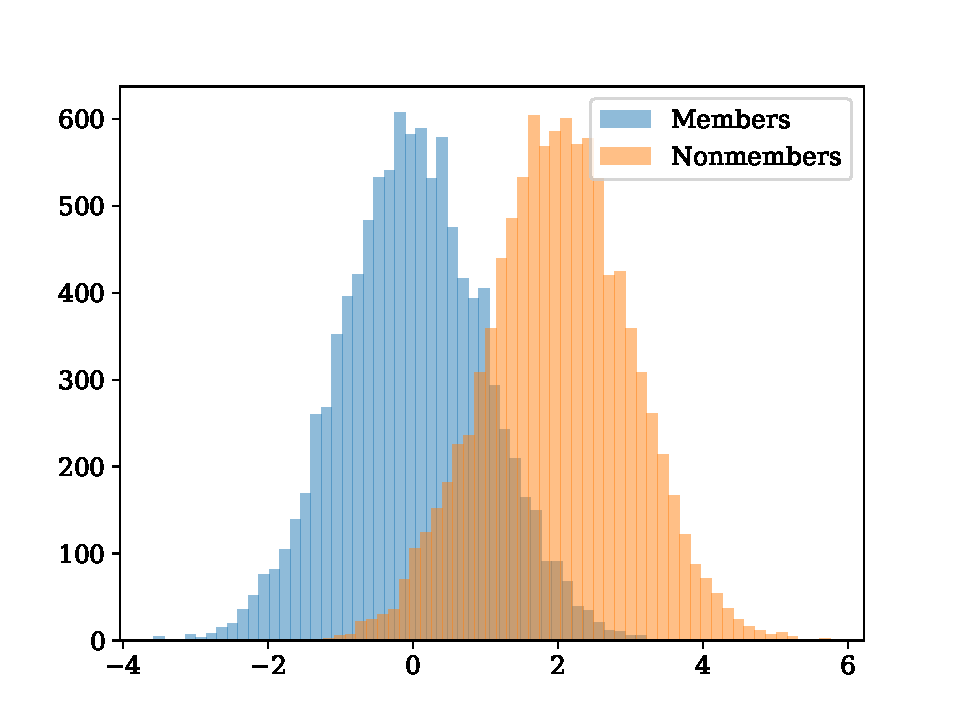
\includegraphics[width=1.05\linewidth,trim={1cm 0 0.5cm 0.5cm}]{images/figures/loss_thrs.pdf}
    \end{center}
    \textbf{Loss Threshold Attack}: $IF\ loss(sample)<threshold\ THEN\ member\ ELSE\ nonmember$.
}


        % --------------------------------- Approaches  ----------    

        \block{\textsc{Problem: lack of nonmembers set}}{
    \textit{We cannot run MIA evaluation without nonmembers}. A few approaches has been proposed:
    \begin{enumerate}{
        \item Fine-tune Stable Diffusion on a new dataset\cite{duan2023diffusion}. \textbf{Pitfall}: too trivial problem due to overfitting.
        \item Train a new model on a new dataset. \textbf{Problem}: too expensive.
        \item Create a dataset with similar properties to the original one. \textbf{Challenge}: distribution mismatch.
    }\end{enumerate}
}



        % ---------------------------------  POKEMON Teaser ----------

        \block{\textsc{Pitfall: Fine-tuning}}{
    \begin{center}
        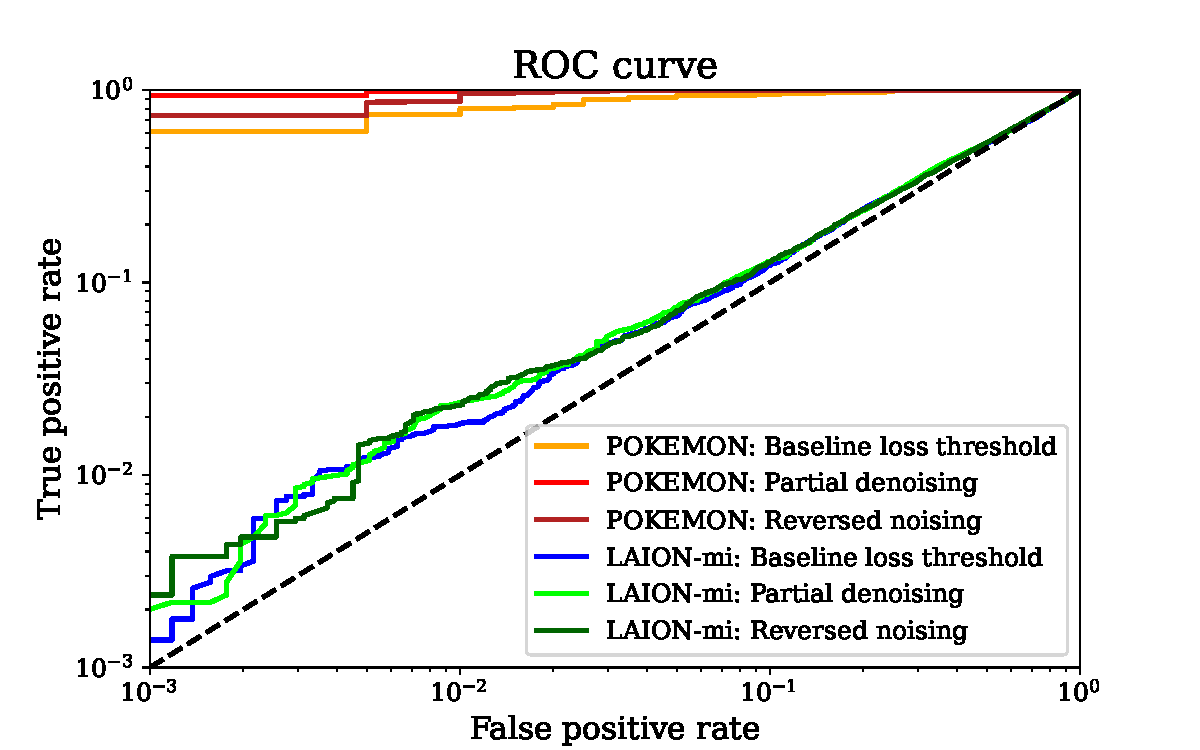
\includegraphics[width=1.05\linewidth]{images/figures/teaser.pdf}
    \end{center}
    Pitfalls in the evaluation setting can lead to incorrect conclusions on the effectiveness of \textit{membership inference attacks} against large diffusion models such as Stable Diffusion.
}


        
        %%%%%%%%%%%%%%% Column 2 %%%%%%%%%%%%%

        \subcolumn{.33}

        % --------------------------------- PARTIE 4  ----------
        
        \block{\textsc{Placeholder}}{
    A placeholder
}



        % ------------------------------------ LAION-mi dataset ------------
        
        \block{\textsc{LAION-mi Dataset}}{
    \begin{center}
        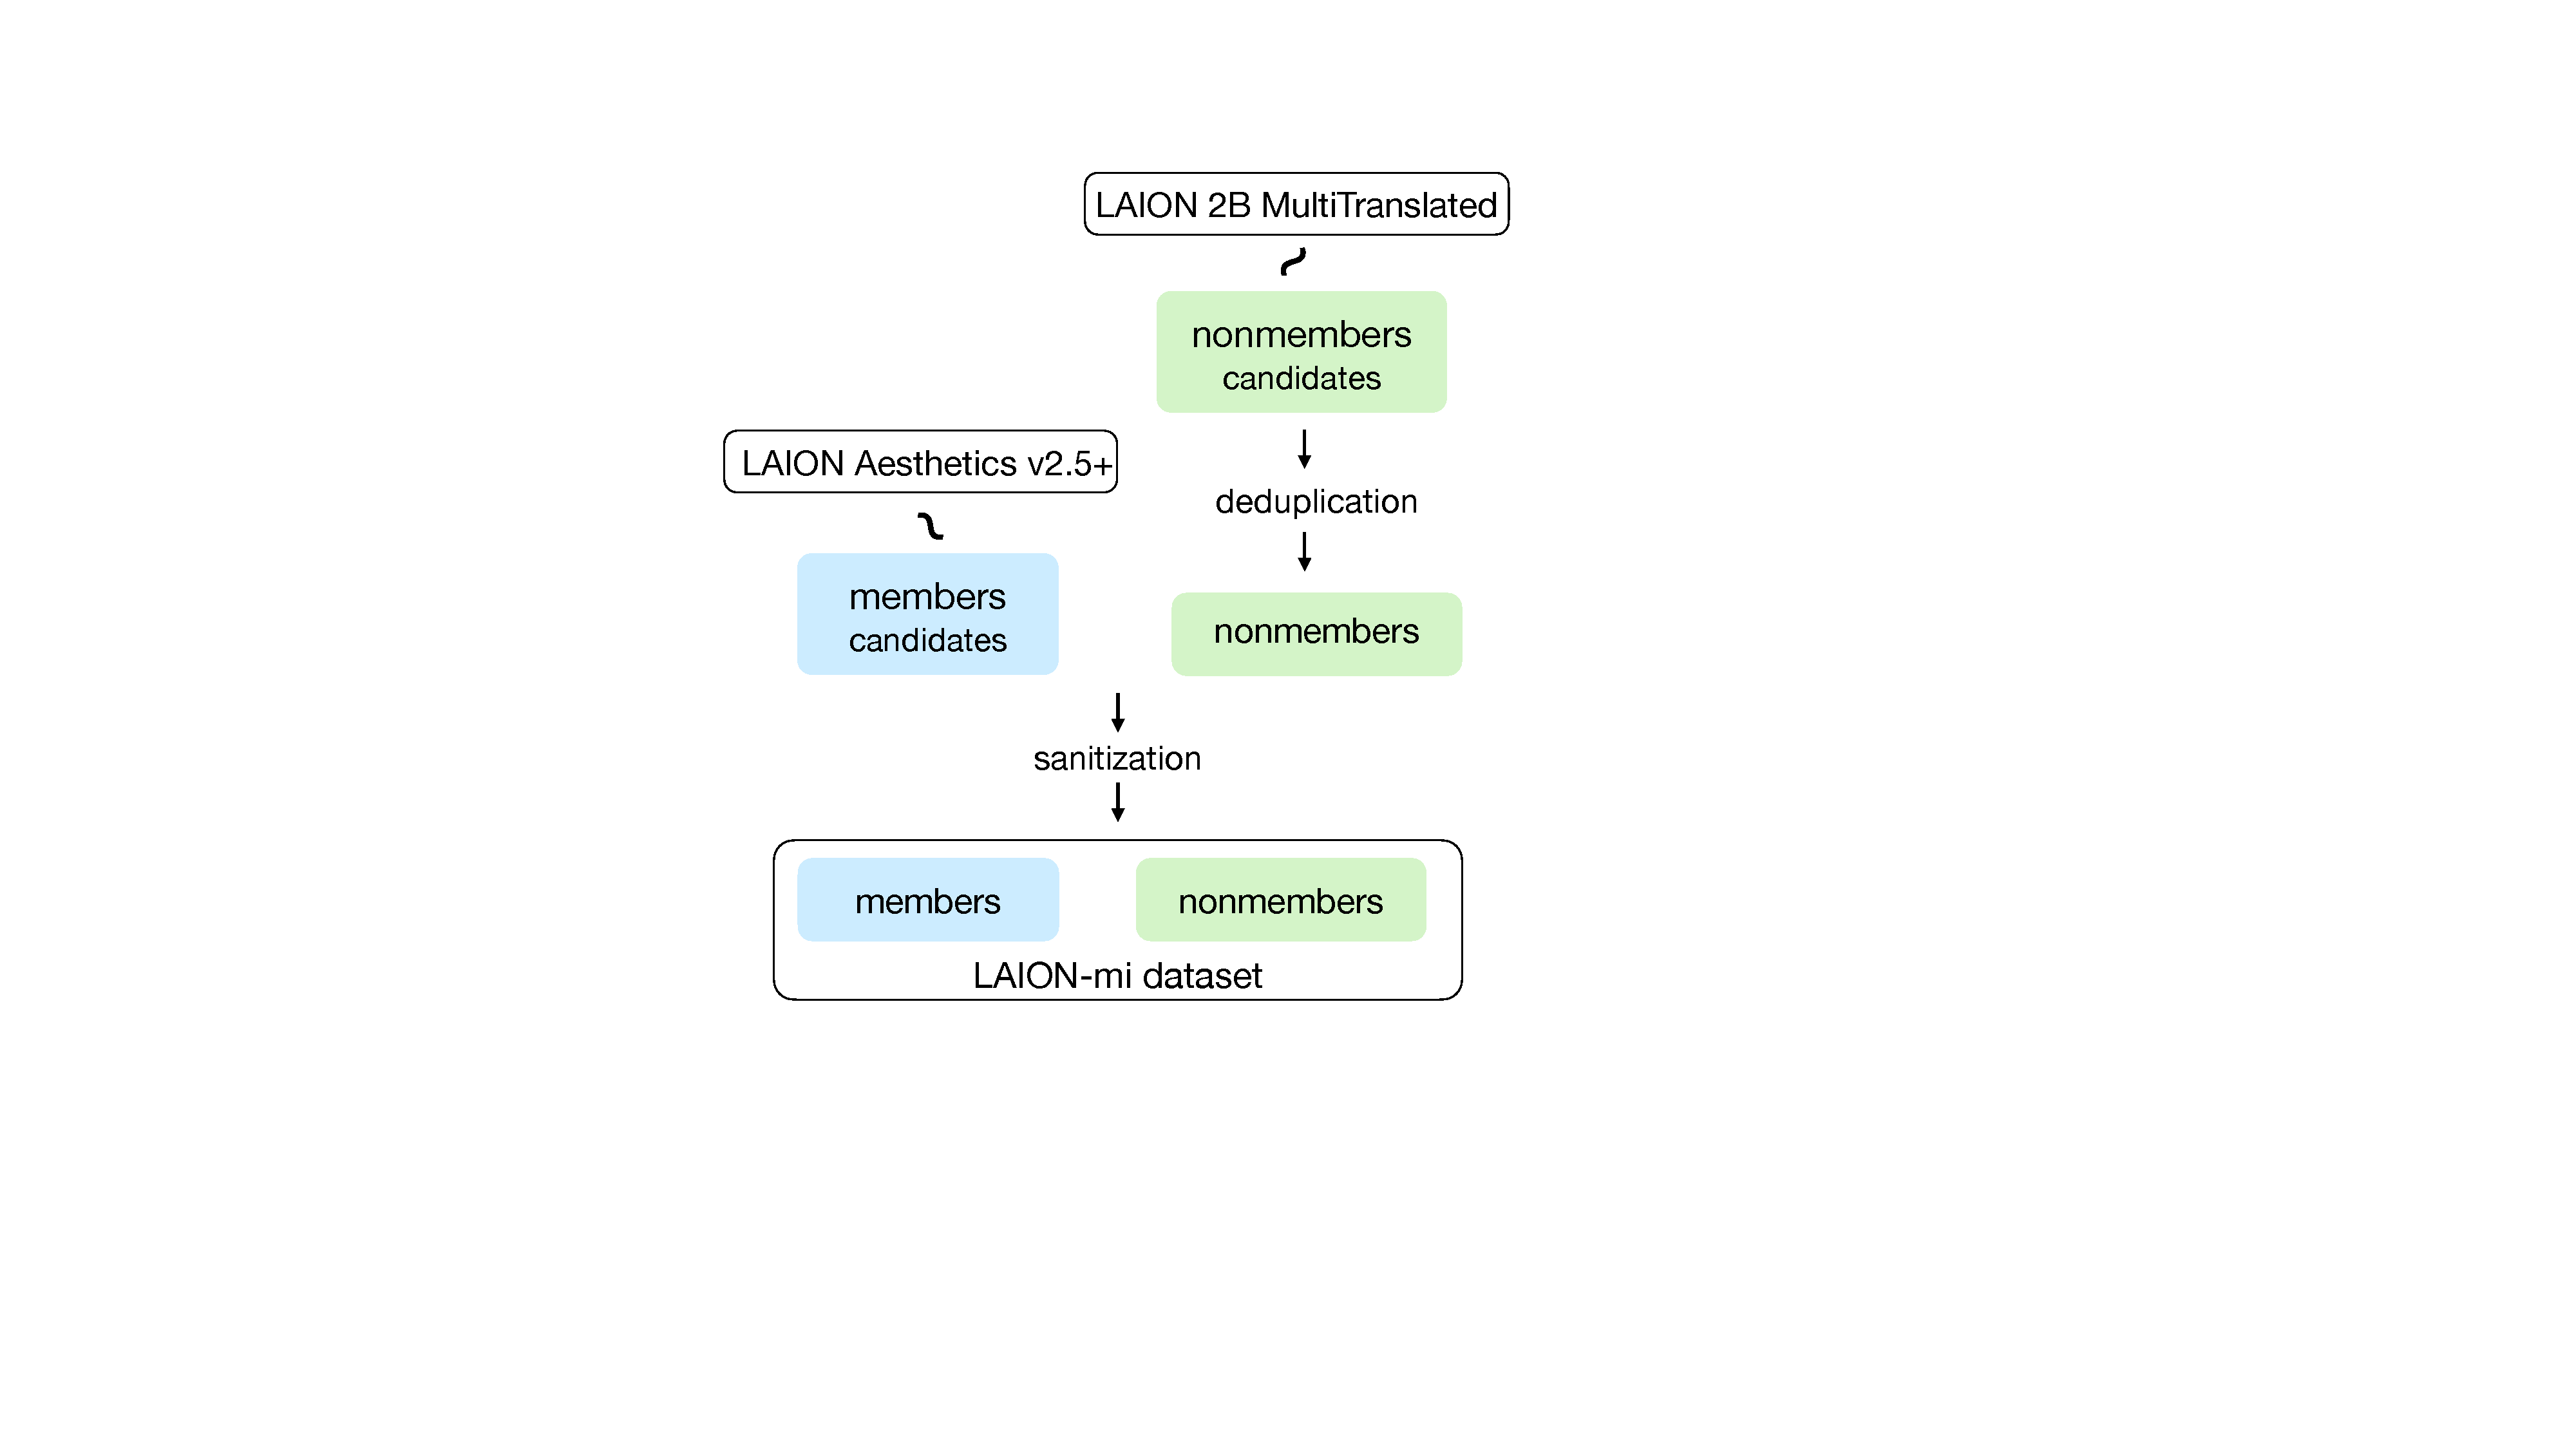
\includegraphics[width=\linewidth]{images/figures/LAION-mi-scheme_3.pdf}
    \end{center}
    A general scheme of constructing LAION-mi dataset.
}



        % ------------------------------------ Challenges ------------
        
        \block{\textsc{Placeholder}}{
    A placeholder
}



        % ------------------------------------ Deduplication plots ------------
        
        \block{\textsc{Placeholder}}{
    A placeholder
}



        % ------------------------------------ QR code to paper ------------
        
        \block{\textsc{Placeholder}}{
    A placeholder
}



        %%%%%%%%%%%%%%%%%%%%%%%% Column 3 %%%%%%%%%%%%%%%%%%%%%%%%%   

        \subcolumn{.33}

        % ------------------------------------ Distribution check ------------
        
        \block{\textsc{Placeholder}}{
    A placeholder
}



        % ------------------------------------ PCA plots ------------
        
        \block{\textsc{Placeholder}}{
    A placeholder
}



        % ------------------------------------ FID table ------------
        
        \block{\textsc{Placeholder}}{
    A placeholder
}



        % ------------------------------------ LAION-mi pics ------------
        
        \block{\textsc{Placeholder}}{
    A placeholder
}



        % ------------------------------------ Evaluation table ------------
        
        \block{\textsc{Placeholder}}{
    A placeholder
}



    \end{subcolumns}


    % ---------------------------------  References ----------
    \block{}{\vspace{1cm}
        \printbibliography}
\end{columns}

% ----------------- Footer -------------
\node [above right, text=white,outer sep=45pt,minimum width=\paperwidth, align=center, draw, fill=titledarkcolor, color=Orange] at (-43.6,-61) { \textcolor{white}{\normalsize Contact: prenom.nom@univ-lyon2.fr}};

\end{document}
